\labday{Lunes, 1 Septiembre 2014}
\experiment{Sistema de gestión de versiones: Git}

Puesta en marcha del sistema de gestión de versiones Git: \url{http://git-scm.com/}.
Ver también: \url{http://en.wikipedia.org/wiki/Git_%28software%29}\\
Para poder trabajar de manera colaborativa se utiliza el servidor remoto
de github \url{https://github.com/}. Este servicio es gratis para repositorios 
que permanezcan abiertos a todo el publico. También, presenta el beneficio de 
plantear un marco para poder compartir desarrollos y códigos de manera libre.
En particular en este desarrollo se opto por una licencia GPL v2.

El esquema del repositorio es el siguiente:
\dirtree{%			
.1 Sensor-Temperatura/ \DTcomment{Directorio Raiz}.
.2 DailyLog/ \ldots{} \begin{minipage}[t]{5cm}
			  Este directorio contiene el \LaTeX\ del diario 
			  de desarrollo(*.tex ){.}
		      \end{minipage}.
.3 dailyLog.tex \DTcomment{Archivo principal}.
.3 Sep.
.4 1-4.tex \DTcomment{Archivo Semanal}.
.3 Oct.
.4 1-4.tex.
.3 Nov.
.4 1-4.tex.
.2 Doc \ldots{} \begin{minipage}[t]{5cm}
			  En este directorio se encuentra toda la documentación utilizada 
			  durante el desarrollo{.}
		      \end{minipage}.
.3 Datasheets.
.3 Lista de Componentes.
.2 Design \ldots{} \begin{minipage}[t]{5cm}
			  Directorio destinado a los diseños de esquemáticos
			  y PCB{.}
		      \end{minipage}.
.3 LM35.
.4 LM35-Remote.sch \DTcomment{Esquemático}.
}


\experiment{Selección de sensor de temperatura}
Para la selección del sensor se tuvo en cuenta principalmente el material disponible.
De esta manera las posibilidades de un sensor de temperatura que se pueden encontrar 
en el mercado local se reducen a:
\begin{itemize}
 \item LM335
 \item LM35
 \item Termistores comunes (1~10K)
\end{itemize}
Las hojas de datos(Datasheets) de los componentes LM335 y LM35 se encuentran en el directorio
$Doc/$. Por otro lado los termistores son dejados como segundas opciones debido a que no son
lineales como los dos anteriores, lo que representa una mayor complejidad en el ajuste de la 
curva y una posible perdida de precisión. 
Ver: \url{http://es.wikipedia.org/wiki/Termistor#Introducci.C3.B3n}

Ambos sensores son analógicos con salidas en voltaje.
\begin{table}[H]
  \begin{tabular}{l l l}
    \toprule
    \textbf{Sensor} & \textbf{Factor de escala} & \textbf{Rango de operación} \\
    \toprule
    LM335 & $10mV/^o K$ & $-40~a~100 ^o C$\\
    LM35  & $10mV/^o C$ & $-55~a~150 ^o C$\\
    \bottomrule
  \end{tabular}
  \caption{Comparación de los sensores LM335 y LM35}
  \label{tab:compSens}
\end{table}

Como podemos observar de la Tabla \ref{tab:compSens} el sensor $LM35$ presenta beneficios 
en cuanto al rango y no es necesaria la conversión de $^o K$ a $^o C$ no requiriendo la
sustracción de una gran constante de voltaje. Por tales motivos se opta por utilizar el
$LM35$ como sensor para el proyecto.

\experiment{Pre selección de PIC 18Fxx}
Se desea tener un sistema en el que un nodo central(beagleBone) se comunique con nodos esclavos
los cuales deben ser capaces de medir la temperatura de 3 a 6 puntos diferentes. La comunicación
entre nodos es digital y es el nodo esclavo el encargado de la conversión analógica/digital
y de la transmisión al nodo central.

Estas razones nos llevan a elegir un micro-controlador con los suficientes canales ADC para
poder realizar la conversión y un UART para la transmisión digital de los datos. Los PIC de 
la familia $18Fxx$ presentan características que los hacen interesantes para este proyecto.

%--------------------------------------------------
\labday{Martes, 2 Septiembre 2014}
\experiment{Topologia de un nodo esclavo}
Para cumplir con las siguientes condiciones del proyecto:
\begin{itemize}
 \item Multiples puntos de sensado
 \item Distancias variables entre los puntos y el nodo central.
 \item Numero variable de puntos.
\end{itemize}
Se opta por utilizar una topologia como la que se observa en la Fig.
\todo{hacer dibujo de la topologia de un nodo esclavo}
De esta manera el nodo esclavo es capaz de sensar un numero $x$ de puntos, cercanos al mismo
y transmitirlos de manera digital al nodo central, de manera que la distancia no sea un factor 
tan influyente. Ademas, este sistema permite la utilización de un bus de comunicación, haciendo 
que el mismo pueda ser escalable, adaptándose fácilmente a un mayor numero de
puntos de medida.
\experiment{Compra de componentes}
\todo{Hacer la lista de las compras hechas en electrónica mendoza}
Se compraron los siguientes elementos en Electrónica~Mendoza.
\begin{table}[H]
  \begin{tabular}{l l l}
    \toprule
    \textbf{Cantidad} & \textbf{Descripción} & \textbf{Importe} \\
    \toprule
    6 	& 	Cable UTP 	& 	36\\
    10  & 	1n4148		& 	2\\
    2	&	18F2550		&	193\\
    15	&	Resistencia	&	3.75\\
    50	&	Resistencia	&	6\\
    1	&	18F4550		&	101.96\\
    5	&	LM35		&	120\\
    3	&	LM317		&	17.10\\
    9	&	Potenciometros	&	42.38\\
    2	&	LM385		&	30.60\\
    10	&	Capacitor	&	4.10\\

    \bottomrule
  \end{tabular}
  \caption{Compras del día 2 de Septiembre}
  \label{tab:compra}
\end{table}
Lo que hace un total de $\$557.61$


%--------------------------------------------------
% Miercoles 3
%--------------------------------------------------
\labday{Miércoles, 3 Septiembre 2014}

\experiment{Esquema de conexión del LM35 (Sensor de temperatura)}
Debido a que los sensores se pueden encontrar a una distancia considerable del nodo esclavo, 
se debe diseñar una manera de poder llevar la señal analógica hasta el micro-controlador. 
Para ello se opta por un esquema como el que se observa en la Fig.\ref{fig:LM35_4_20mA}

\begin{figure}[H] % Example of including images
  \begin{center}
  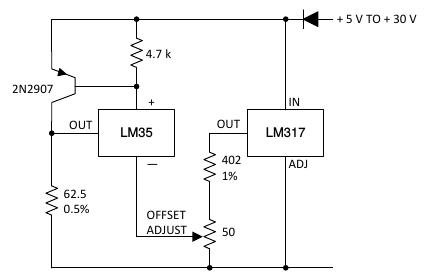
\includegraphics[width=0.5\linewidth]{LM35_4_20mA}
  \end{center}
  \caption{Esquema de conexión del LM35 (4 a 20 mA) }
  \label{fig:LM35_4_20mA}
\end{figure}

Con este tipo de conexión convertimos nuestra señal de tensión a una de corriente de $4$ a $20mA$.
Lo que nos asegura poder transmitir durante mayores distancias.
Detallamos a continuación el funcionamiento de cada una de las partes del circuito:
\begin{itemize}
 \item LM35:\\ 
    Tiene a su salida una tensión proporcional a la temperatura. De manera que en $OUT$
    tendremos $10mV/^oC$. Al pasar por la resistencia se convierte en una corriente 
    proporcional a $I_{out}=\dfrac{V_{out}}{R_{62.5}}$. Como el negativo esta conectado
    con una resistencia a un regulador de tensión nos permite ajustar la escala. 
 \item LM317: \\
    En su salida la tensión regulada que cambia el offset del LM35. Y la corriente se suma
    a la del LM35. 
 \item Transistor PNP:\\
    (Ver: \url{http://es.wikipedia.org/wiki/Transistor_de_uni%C3%B3n_bipolar})
    La resistencia de $4.7K$ permite que la corriente pase por el transistor en ves de por $LM35$
    de esta manera es el transistor el que la entrega cuando $I>=\dfrac{V_{0.6}}{4.7K}$
\end{itemize}
Una ves que tenemos nuestra señal de $4$ a $20mA$ para ser leída por el ADC usamos una resistencia 
de $50 \Omega$ y una $V_{ref}$ para poder cambiar la escala en el $PIC$

\experiment{Prueba del sensor LM35}
Para poder verificar el correcto funcionamiento del integrado realizamos el circuito
de la Fig.\ref{fig:basic_LM35}
\begin{figure}[H] % Example of including images
  \begin{center}
  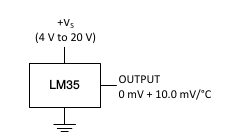
\includegraphics[width=0.5\linewidth]{basic_LM35}
  \end{center}
  \caption{Sensor de temperatura básico}
  \label{fig:basic_LM35}
\end{figure}


Mediante un tester medimos el valor de tensión, el cual nos entrega como resultado 
$230mV$ equivalente a $23^oC$. Esto es coherente y proseguimos con los ensayos sobre este
sensor.

\experiment{Prueba del regulador LM317}
Se realiza el esquema de la Fig.\ref{fig:basic_LM317} para probar si el
controlador responde la manera esperada. Mediante el potenciometro se cambian los valores
de tensión de salida del controlador. Alimentado con $12v$ se consiguen valores desde
$2v$ a $11.5v$. De esta manera se ha verificado que el controlador funciona.

\begin{figure}[H] % Example of including images
  \begin{center}
  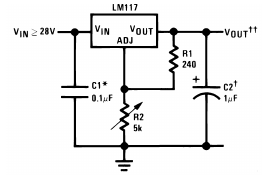
\includegraphics[width=0.5\linewidth]{basic_LM317}
  \end{center}
  \caption{Regulador de tensión típico }
  \label{fig:basic_LM317}
\end{figure}


\experiment{Prueba del Diagrama de la Fig.\ref{fig:LM35_4_20mA}}
No se pudo realizar por falta del transistor PNP $2N2907$

\experiment{Realización del esquemático en EagleCAD}
Se realizo en el software EagleCAD el diagrama de la Fig.\ref{fig:LM35_4_20mA} junto con 
la primera versión del PCB.\todo{agregar captura de pantalla de EagleCAD}

%-----------------------------------------------------
% Jueves 4 Septiembre
%-----------------------------------------------------
\labday{Jueves 4, Septiembre}
\experiment{Compra de los elementos faltantes}
Debido a que el día 3 de Septiembre no se pudo realizar los ensayos por falta de material,
el jueves a la mañana se realizo la compra de los materiales necesarios. Ademas, se sumaron
los materiales para 
\begin{itemize}
 \item La adaptación de una fuente de computadora como fuente de tensión para
los ensayos
\item El desarrollo de los circuitos impresos.
\end{itemize}
 
\begin{table}[H]
  \begin{tabular}{l l l}
    \toprule
    \textbf{Cantidad} & \textbf{Descripción} & \textbf{Importe} \\
    \toprule
    4 	& 	Banana Hembra 	& 	6\\
    4  & 	Banana Macho	& 	12\\
    4	&	Cocodrilo	&	10\\
    1	&	Transferencia	&	35\\
    1	&	Placa Fibra	&	58\\
    20	&	Resistencia	&	2.40\\
    2	&	2N2907		&	9.08\\
    3	&	2N3906		&	3.66\\
    2	&	LM35		&	48\\
    4	&	Unipolar	&	7\\
    1	&	Jac		&	3.86\\
    1	&	Plug		&	5\\
    \bottomrule
  \end{tabular}
  \caption{Compras del día 4 de Septiembre}
  \label{tab:compra}
\end{table}
Lo que hace un total de $\$200$

\experiment{Prueba del Diagrama de la Fig.\ref{fig:LM35_4_20mA}}

Tras realizar los ensayos del circuito de la Fig.\ref{fig:LM35_4_20mA} se observa que 
\begin{itemize}
 \item Los valores de las resistencias deben ser muy específicos para que el sistema funcione
 entre los $4$ a $20mA$. Sobre todo la de $62.5\Omega$ que tiene su valor de 
 $62.5\Omega=\dfrac{1V(Rango~Sensor)}{16mA(Rango~Senal)}$
 \item Al utilizar el regulador $LM317$ obtenemos el desfazaje de escala a los $4mA$ pero 
 agregamos complejidad en el ajuste de las resistencias y calor al sistema de medición.
\end{itemize}

Para poder minimizar el numero de resitencias a ajustar y la complejidad del sistema se 
opta por no utilizar el $LM317$ y conectar directo el $LM35$. Esto nos da una escala que 
arranca $0mA$ para $0^oC$. Luego si utilizamos una resistencia de valor comercial al $0.5\%$
de lamina de metal para que sea mas precisa y menos sensible al calor, tenemos la escala 
$20mA(Rango~Senal)=\dfrac{1V(Rango~Sensor)}{(50\Omega}$. Obteniendo un diagrama como el que
se ve en la Fig.\todo{Agregar diagrama del nuevo circuito}

Finalmente, obtenemos un sistema con menos componentes y que se ajusta por software pero 
que al mismo tiempo es mas repetible. 

\experiment{Prueba del Diagrama nuevo}
Utilizando el nuevo esquematico y las resistencias con las que contamos son:
\begin{itemize}
 \item $46.1\Omega$ para la salida del $LM35$
 \item $217\Omega$ para transformar de corriente a tensión nuevamente.
\end{itemize}

Los resultados que obtenemos son $V=1.19v$ lo cual significa que circula una corriente
$I=\dfrac{1.19v}{217\Omega}=5.5mA$ por lo que el $LM35$ esta entregando 
$V=5.5mA~46.1=0.25v$ lo cual es coherente con la temperatura del lugar.

\experiment{Nueva versión del esquemático en EagleCAD}
Se elimina el uso del LM317 y se conecta por plug en ves de utilizar pines.